%----------------------------------------------------------------------------
\chapter{A mérés}
%----------------------------------------------------------------------------

	A poros plazma kísérleteket jól áttekintő cikk \cite{merlino2006dusty}.

	\begin{figure}[!h]
		\centering
		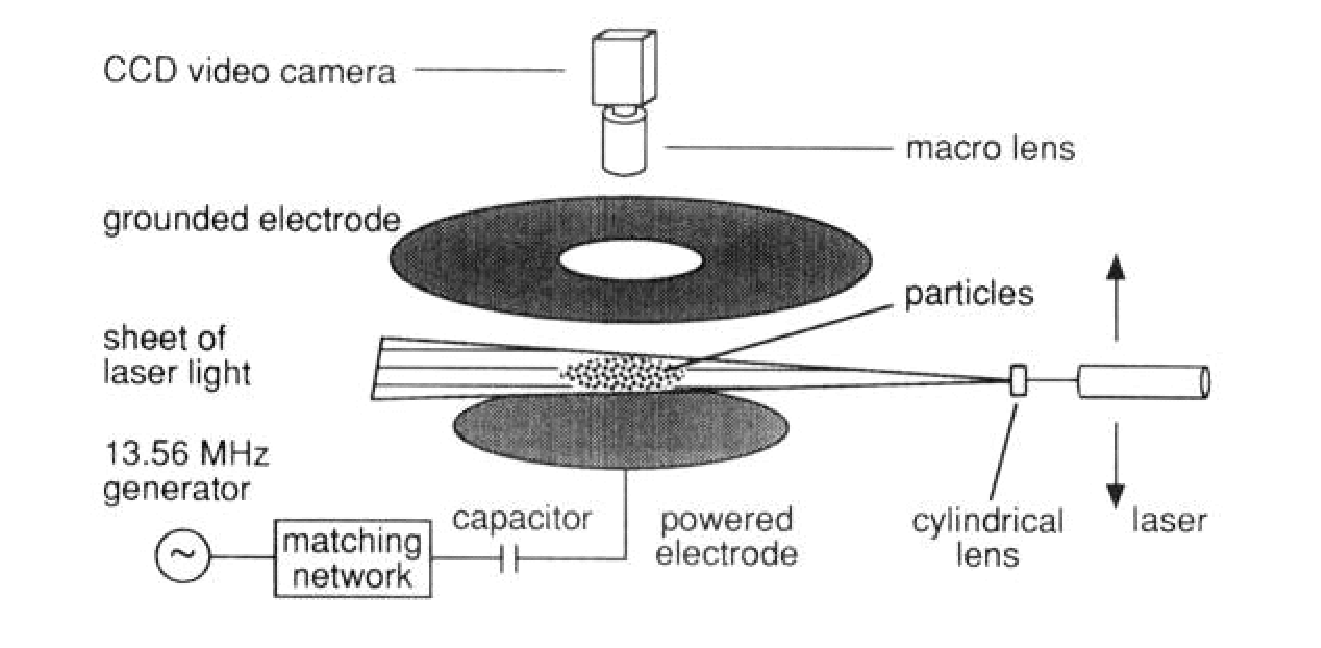
\includegraphics[width=0.9\columnwidth]{figures/eps/dust_camera.eps}
		\caption{A mérési elrendezés sematikus ábrája (forrás: \cite{merlino2006dusty})} 
		\label{fig:device} 
	\end{figure}
	
	\begin{figure}[!h]
		\centering
		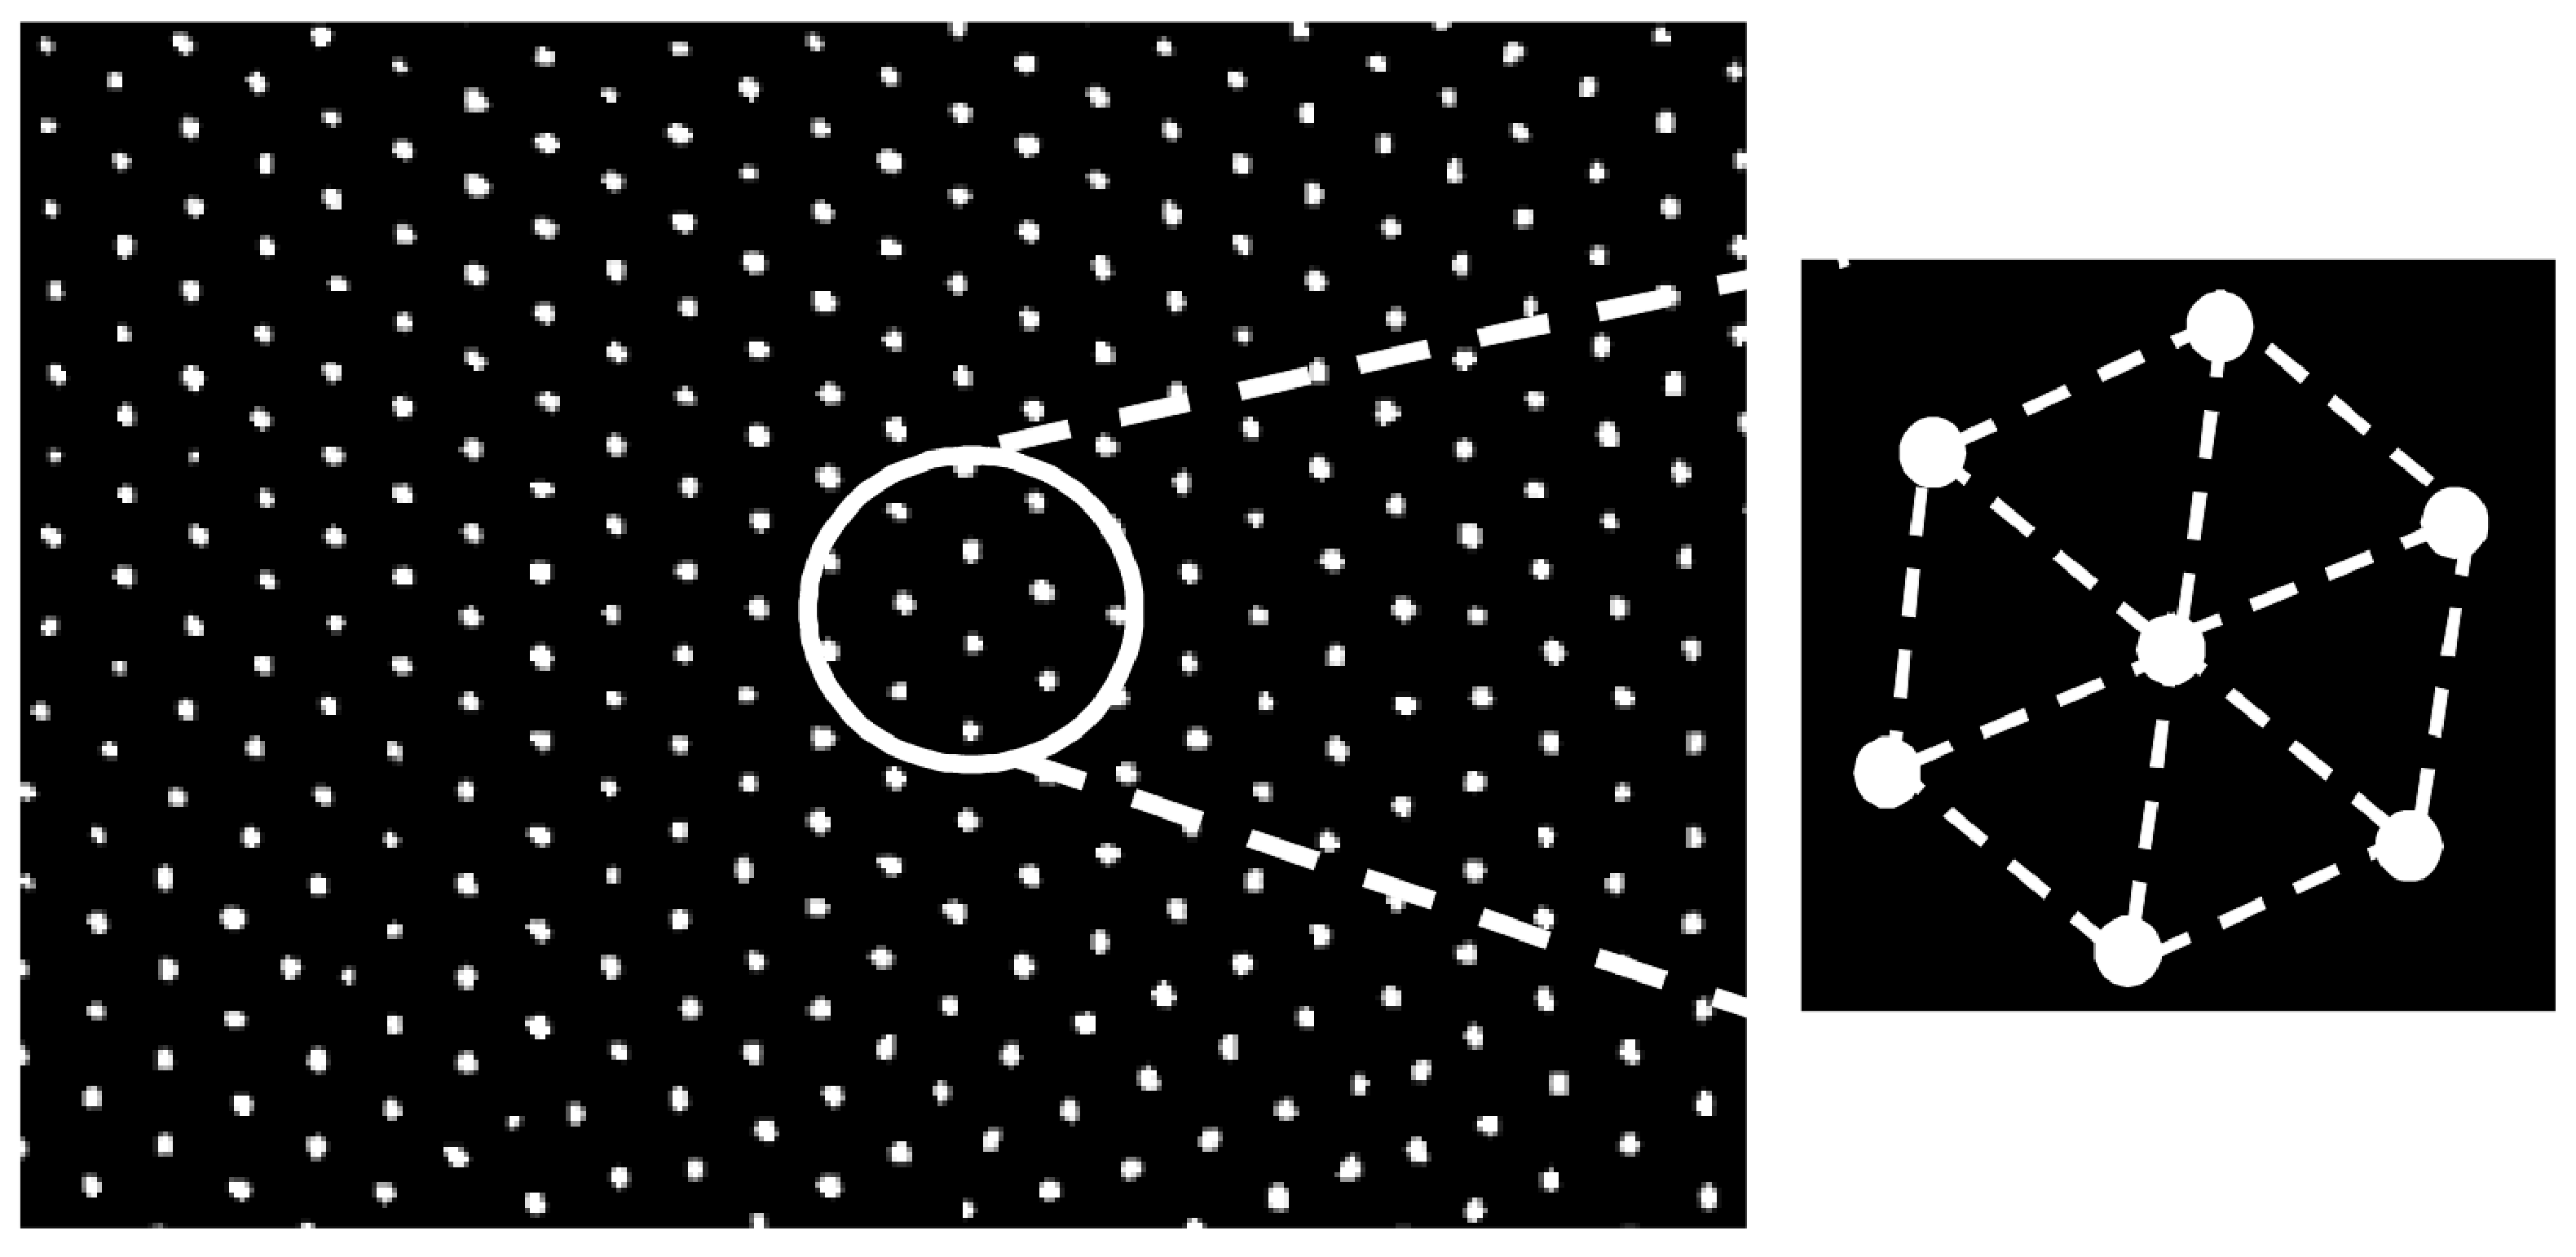
\includegraphics[width=0.9\columnwidth]{figures/eps/coulomb_crystal.eps}
		\caption{2D-s Coulomb kristály hatszögletű struktúrájával (forrás: \cite{merlino2006dusty})} 
		\label{fig:device} 
	\end{figure}


\section{A mérési elrendezés}
%----------------------------------------------------------------------------
	
	\begin{align}
	W(s)=\frac{A}{1+2T\xi s+s^2T^2}.
	\end{align}

%----------------------------------------------------------------------------
\section{A mérendő mennyiségek és a származtatott értékek}
%----------------------------------------------------------------------------










